\section{DIFFERENTIAL DRIVE MOBILE ROBOT MODELING}
\subsection{Mobile Robot Kinematic}
\hspace{1.27cm}
Kinematic model of the robot describes the transformation of the robot velocities in the local frame to the velocity in global frame. Using kinematic model, the robot pose is determined and represented in the coordinate system.
\par

% Figure Image =============================================================================
\begin{figure}[ht]
	\centering
	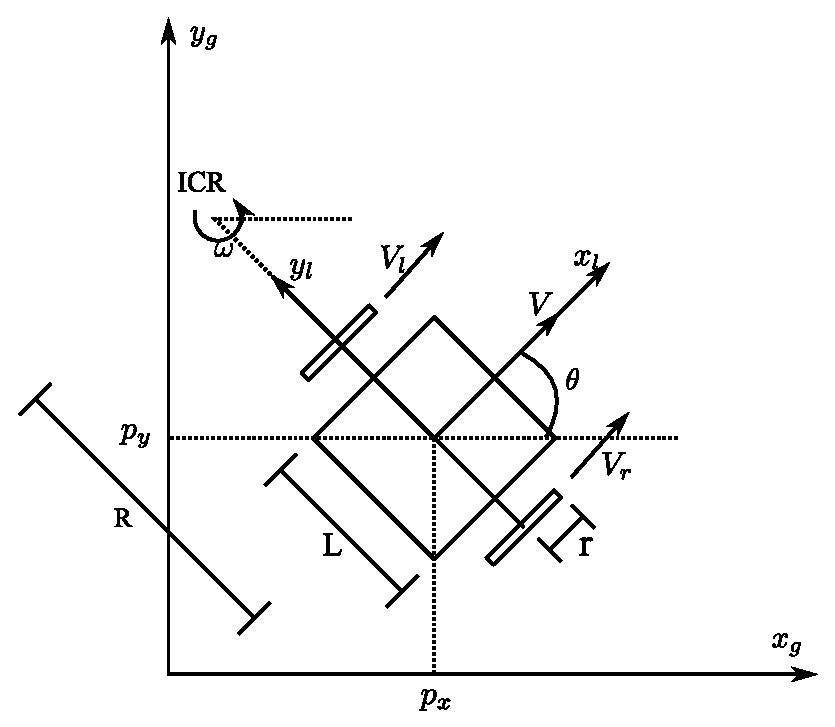
\includegraphics[scale=1]{images/imagess/4dmodel-DDmodeling.eps} 
	\caption{Differential Drive Kinematic Model}
	\label{fig:Differential Drive Kinematic Model}
\end{figure}

% Figure Image =============================================================================
In \textbf{\figureautorefname{ \ref{fig:Differential Drive Kinematic Model}}} Let:
\begin{itemize}
	\item {\makebox[1cm]{\(r\)\hfill} is the radius of the wheel}
	\item {\makebox[1cm]{\(R(t)\)\hfill} is the instantaneous radius of the vehicle driving trajectory}
	\item {\makebox[1cm]{L\hfill} is the length of the robot base}
	\item {\makebox[1cm]{\(V_l\)\hfill} is the linear velocity of the left wheel}
	\item {\makebox[1cm]{\(V_r\)\hfill} is the linear velocity of the right wheel}
	\item {\makebox[1cm]{\(V\)\hfill} is the linear velocity of the robot base}
	\item {\makebox[1cm]{\(\omega\)\hfill} is the angular velocity of the robot base}
	
%	\item \(r\) is the radius of the wheel
%	\item \(R(t)\) is the instantaneous radius of the vehicle driving trajectory
%	\item L is the length of the robot base
%	\item \(V_l\) is the linear velocity of the left wheel
%	\item \(V_r\) is the linear velocity of the right wheel
%	\item \(V\) is the linear velocity of the robot base
%	\item \(\omega\) is the angular velocity of the robot base
\end{itemize}

From \textbf{\figureautorefname{ \ref{fig:Differential Drive Kinematic Model}}}, we obtain:
\begin{equation} \label{eq:MRKi1}
\omega = \frac{V_l(t)}{R(t)-\frac{L}{2}}
\end{equation}
\begin{equation} \label{eq:MRKi2}
\omega = \frac{V_r(t)}{R(t)+\frac{L}{2}}
\end{equation}
\par

From \ref{eq:MRKi1} and \ref{eq:MRKi2}, we get:
\begin{equation} \label{eq:MRKi3}
\omega(t) = \frac{V_r(t)-V_l(t)}{L}
\end{equation}
\begin{equation} \label{eq:MRKi4}
R(t) = \frac{L}{2} \frac{V_r(t)+V_l(t)}{V_r(t)-V_l(t)}
\end{equation}

We have:
\begin{equation} \label{eq:MRKi5}
V(t) = R(t)\omega(t)
\end{equation}

Substitute \ref{eq:MRKi3} and \ref{eq:MRKi4} to \ref{eq:MRKi5}, we get:
\begin{equation}
V(t) = \frac{V_r(t)+V_l(t)}{2}
\end{equation}


We know:
\begin{equation}
\begin{split} \label{eq:MRKi6}
V_l(t) = r\omega_l(t)\\
V_r(t) = r\omega_r(t)
\end{split}
\end{equation}

Substitute \ref{eq:MRKi6} to \ref{eq:MRKi5} and \ref{eq:MRKi3}, we get:
\begin{equation} \label{eq:MRKi_V}
V(t) = \omega_r \frac{r}{2} + \omega_l \frac{r}{2}
\end{equation}
\begin{equation} \label{eq:MRKi_omega}
\omega(t) = \omega_r \frac{r}{L} - \omega_l \frac{r}{L}
\end{equation}


Robot kinematic model in global frame is defined as:
\begin{equation} \label{eq:MRKi7}
\begin{bmatrix}
\Dot{p_x} \\
\Dot{p_y} \\
\Dot{\theta}
\end{bmatrix} = 
\begin{bmatrix}
cos(\theta) && 0\\
sin(\theta) && 0\\
0 && 1
\end{bmatrix}
\begin{bmatrix}
V(t)\\
\omega(t)
\end{bmatrix}
\end{equation}

Using Euler integration, the equation of motion in discrete time form is:
\begin{equation}
\begin{bmatrix}
p_{x,k}\\
p_{y,k}\\
\theta_{k}\\
\end{bmatrix}=
\begin{bmatrix}
p_{x,k-1} + V_{k-1} T_s cos(\theta_{k-1}) \\
p_{y,k-1} + V_{k-1} T_s sin(\theta_{k-1}) \\
\theta_{k-1} + \omega_{k-1} T_s\\
\end{bmatrix}
\end{equation}
Where:
\begin{itemize}
	\item {\makebox[1cm]{k\hfill} is the time step}
	\item {\makebox[1cm]{\(T_s\)\hfill} is the time interval}
%    \item k is the time step
%    \item \(T_s\) is the time interval
\end{itemize}




\subsection{Mobile Robot Dynamics}
\hspace{1.27cm}
Differential drive mobile robot is a dynamics system. Using solely the kinematic model of the system is not enough to represent the system as a whole. For the robustness of the robot, the dynamics properties of the system such as external force, mass, inertia are considered. In our case the robot center of mass is coincides with the center geometric of the robot. Let \(m\) be the mass of the robot, \(J\) be the moment of inertia of the robot about Z-axis. In this section, we use q to describe the generalized coordinate of the system \(q=[x, y, \theta]\) and \(\tau_l\) is the left wheel torque, \(\tau_r\) is the right wheel torque.\par

The dynamics model of the robot with constraint is derived using Lagrange formulation:
\begin{equation}{\label{eq:lagrangain eq full}}
\frac{\partial}{\partial t}(\frac{\partial \mathcal{L}}{\partial \Dot{q}_k})- \frac{\partial \mathcal{L}}{\partial q_k} + \frac{\partial P}{\partial \Dot{q}_k} + g_k + \tau_{dk}= f_k - \sum_{j=1}^{m}\lambda_j a_{jk}
\end{equation}
Where:
\begin{itemize}
	\item {\makebox[1cm]{\(\mathcal{L}\)\hfill} is the Lagrangian}
	\item {\makebox[1cm]{\(P\)\hfill} is the power dissipation function due to friction and damping}
	\item {\makebox[1cm]{\(g_k\)\hfill} are the forces due to gravitation}
	\item {\makebox[1cm]{\(\tau_{dk}\)\hfill} are the system disturbances}
	\item {\makebox[1cm]{\(f_k\)\hfill} are the general forces (external influences to the system)}
	\item {\makebox[1cm]{\(q_k\)\hfill} general coordinate k=(1,...,n)}
	\item {\makebox[1cm]{m\hfill} is the number of linearly independent motion constraint}
	\item {\makebox[1cm]{\(\lambda_j\)\hfill} is the Lagrange multiplier associated with the jth constraint relation}
	\item {\makebox[1cm]{\(a_{jk}\)\hfill} is coefficients of the constraints (j=1,...,n)}
	
%    \item \(\mathcal{L}\) is the Lagrangian
%    \item \(P\) is the power dissipation function due to friction and damping
%    \item \(g_k\) are the forces due to gravitation
%    \item \(\tau_{dk}\) are the system disturbances
%    \item \(f_k\) are the general forces (external influences to the system)
%    \item \(q_k\) general coordinate k=(1,...,n)
%    \item m is the number of linearly independent motion constraint
%    \item \(\lambda_j\) is the Lagrange multiplier associated with the jth constraint relation
%    \item \(a_{jk}\) is coefficients of the constraints (j=1,...,n)
\end{itemize}

Assumption:
\begin{itemize}
	\item {\makebox[1cm]{\(\mathcal{W}_p\)\hfill} = 0, the robot is driven on the plane where the potential energy is constant}
	\item {\makebox[1cm]{\(gk\)\hfill} = 0, the robot is driven on the plane where the potential energy is constant}
	\item {\makebox[1cm]{\(\tau_{dk}\)\hfill} = 0, no outside disturbances}
	
%    \item \(\mathcal{W}_p = 0\), the robot is driven on the plane where the potential energy is constant
%    \item \(gk = 0\), the robot is driven on the plane where the potential energy is constant
%    \item \(\tau_{dk}=0\), no outside disturbances
\end{itemize}

The Lagrangian \(\mathcal{L}\) is the difference between kinetic energy and potential energy. We get:
\begin{equation}
\mathcal{L} = \mathcal{W}_k - \mathcal{W}_p 
\end{equation}
Where:
\begin{itemize}
	\item {\makebox[1cm]{\(\mathcal{W}_k\)\hfill} is the kinetic energy of the system}
	\item {\makebox[1cm]{\(\mathcal{W}_p\)\hfill} is the potential energy of the system}
	
%    \item \(\mathcal{W}_k\) is the kinetic energy of the system
%    \item \(\mathcal{W}_p\) is the potential energy of the system
\end{itemize}

The Kinetic energy equation is:
\begin{equation}
\mathcal{W}_k = \frac{1}{2}mV^2 + \frac{1}{2} J\Dot{\theta}^2
\end{equation}

The velocity in the 2D plane is:
\begin{equation}
V^2 = \Dot{x}^2 + \Dot{y}^2
\end{equation}

We get the Lagrangian \(\mathcal{L}\):
\begin{equation}
\mathcal{L} = \frac{m}{2}(\Dot{x}^2 + \Dot{y}^2) + \frac{J}{2}\Dot{\theta}^2
\end{equation}

Substitute back to \ref{eq:lagrangain eq full}, we get:
\[\frac{\partial}{\partial t}(\frac{\partial \mathcal{L}}{\partial \Dot{x}}) = m\Ddot{x}\] 
\[\frac{\partial}{\partial t}(\frac{\partial \mathcal{L}}{\partial \Dot{y}}) = m\Ddot{y}\] 
\[\frac{\partial}{\partial t}(\frac{\partial \mathcal{L}}{\partial \Dot{\theta}}) = J\Ddot{\theta}\]
\[\frac{\partial \mathcal{L}}{\partial x} = 0\] 
\[\frac{\partial \mathcal{L}}{\partial y} = 0\] 
\[\frac{\partial \mathcal{L}}{\partial \theta} = 0\] 

The mobile robot constraint in x-axis is \(-sin\theta\), in y-axis is \(cos\theta\).\\
From \ref{eq:lagrangain eq full}, we obtain:
\begin{equation}
\begin{split}
m\Ddot{x} = F_x - \lambda_1(-sin\theta) \\
m\Ddot{y} = F_y - \lambda_1(cos\theta)\\
J\Ddot{\theta} = M_z
\end{split}
\end{equation}

We get:
\begin{equation}
\begin{split}
m\Ddot{x} - \lambda_1 sin \theta= F_x\\
m\Ddot{y} + \lambda_1 cos \theta= F_y\\
J\Ddot{\theta} = M_z
\end{split}
\end{equation}

Since the assumption of no outside disturbance force, the force acting on the robot are the left wheel force \(F_l\) and the right wheel force \(F_r\). The resultant for is:
\begin{equation}
F = F_r + F_l
\end{equation}

We have:
\begin{equation}
\begin{split}
F_r = \frac{\tau_r}{r}\\
F_l = \frac{\tau_l}{r}
\end{split}
\end{equation}

And
\begin{equation}
\begin{split}
F_x &= F cos\theta \\
F_y &= F sin\theta \\
M_z &= F_r \frac{L}{2} - F_l \frac{L}{2}
\end{split}
\end{equation}

We get:
\begin{equation}
\begin{split}
F_x &= \frac{1}{r} (\tau_r + \tau_l) cos \theta \\
F_y &= \frac{1}{r} (\tau_r + \tau_l) sin \theta \\
M_z &= \frac{L}{2r} (\tau_r - \tau_l)
\end{split}
\end{equation}

We get:
\begin{equation}
\begin{split}
m\Ddot{x} - \lambda sin \theta - \frac{1}{r} (\tau_r + \tau_l) cos \theta = 0\\
m\Ddot{y} + \lambda cos \theta - \frac{1}{r} (\tau_r + \tau_l) sin \theta = 0\\
J\Ddot{\theta} - \frac{L}{2r} (\tau_r - \tau_l) = 0
\end{split}
\end{equation}

Rewrite the equation into Matrix form of:
\[M(q)\Ddot{q} + V (q,\Dot{q}) + F(\Dot{q}) = E(q)u - A^T(q) \lambda\]
We get:
\[M=\begin{bmatrix}
m && 0 && 0\\
0 && m && 0\\ 
0 && 0 && J
\end{bmatrix}\]

\[E=\frac{1}{r}\begin{bmatrix}
cos\theta && cos\theta \\
sin\theta && sin\theta \\ 
\frac{L}{2} && -\frac{L}{2} 
\end{bmatrix}\]

\[A=\begin{bmatrix}
-sin\theta && cos\theta && 0
\end{bmatrix}\]

\[u=\begin{bmatrix}
\tau_r\\
\tau_l 
\end{bmatrix}\]

Where remain are Zero\newline
In the state-space model:

\[\Tilde{M}=\begin{bmatrix}
m && 0 \\
0 && j
\end{bmatrix}\]

\[\Tilde{V}=\begin{bmatrix}
0\\
0
\end{bmatrix}\]

\[\Tilde{E}=\frac{1}{r}\begin{bmatrix}
1 && 1 \\
\frac{L}{2} && -\frac{L}{2} \\ 
\end{bmatrix}\]

The model is
\begin{equation}
\begin{bmatrix}
\Dot{x}\\
\Dot{y}\\
\Dot{\theta}\\
\Dot{V}\\
\Dot{\omega}
\end{bmatrix}=
\begin{bmatrix}
V cos\theta\\
V sin\theta\\
\omega\\
0\\
0
\end{bmatrix}+
\begin{bmatrix}
0&& 0 \\
0&& 0 \\
0&& 0 \\
\frac{1}{mr}&& \frac{1}{mr} \\
\frac{L}{2Jr}&&-\frac{L}{2Jr}
\end{bmatrix}\begin{bmatrix}
\tau_r\\
\tau_l
\end{bmatrix}
\end{equation}

%Using Inverse Model gives the required torque for each wheel to be calculated
%\begin{equation}
%\begin{bmatrix}
%\tau_r\\
%\tau_l
%\end{bmatrix}=
%\begin{bmatrix}
%\frac{\Dot{V}mr}{2} + \frac{\Dot{\omega}Jr}{L}\\
%\frac{\Dot{V}mr}{2} - \frac{\Dot{\omega}Jr}{L}
%\end{bmatrix}
%\end{equation}